\newcolumntype{?}{!{\vrule width 1pt}}

% \newcolumntype{M}[1]{>{\centering\arraybackslash}m{#1}}
% \newcommand\scalefactorqual{0.085}
% \newcommand\spacerqual{3mm}

\begin{figure*}[t!]
    \centering
    \setkeys{Gin}{width=\linewidth}
    \renewcommand\tabularxcolumn[1]{>{\Centering}m{\sfac\linewidth}} % set all columns to be centered v & hwise, with a fixed width
    % \begin{tabularx}{\textwidth}{m{15pt}*{5}{X} @ {\hspace{\spacerqual}}*{5}{X}}%
    % \begin{tabularx}{\textwidth}{m{15pt}*{5}{X}}
    \begin{tabularx}{\textwidth}{m{50pt}*{5}{X}}
        
    \includegraphics{ours_sup/animal_pose_fits/orig/2007_000063.jpg} &
    \includegraphics{ours_sup/animal_pose_fits/fit/2007_000063.jpg} &
    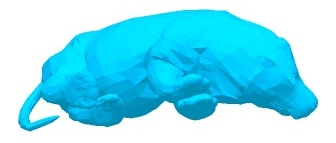
\includegraphics{ours_sup/animal_pose_fits/model/2007_000063_crop.jpg} &
    \includegraphics{ours_sup/animal_pose_fits/joints/2007_000063.jpg} &
    \includegraphics{ours_sup/animal_pose_fits/segs/2007_000063.jpg} \\
    %\hspace{\spacercomp} 
    \includegraphics{ours_sup/animal_pose_fits/orig/2007_004189.jpg} &
    \includegraphics{ours_sup/animal_pose_fits/fit/2007_004189.jpg} &
    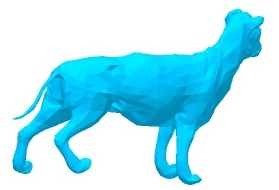
\includegraphics{ours_sup/animal_pose_fits/model/2007_004189_crop.jpg} &
    \includegraphics{ours_sup/animal_pose_fits/joints/2007_004189.jpg} &
    \includegraphics{ours_sup/animal_pose_fits/segs/2007_004189.jpg} \\ 

    % R12
    \includegraphics{ours_sup/animal_pose_fits/orig/2007_008222.jpg} &
    \includegraphics{ours_sup/animal_pose_fits/fit/2007_008222.jpg} &
    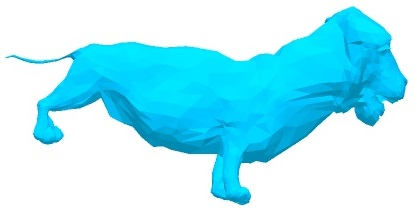
\includegraphics{ours_sup/animal_pose_fits/model/2007_008222_crop.jpg} &
    \includegraphics{ours_sup/animal_pose_fits/joints/2007_008222.jpg} &
    \includegraphics{ours_sup/animal_pose_fits/segs/2007_008222.jpg} \\
    %\hspace{\spacercomp} 
    \includegraphics{ours_sup/animal_pose_fits/orig/2007_009605.jpg} &
    \includegraphics{ours_sup/animal_pose_fits/fit/2007_009605.jpg} &
    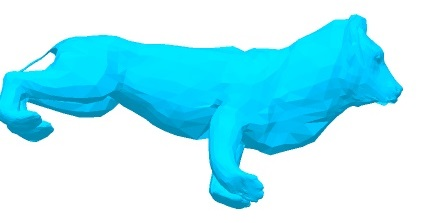
\includegraphics{ours_sup/animal_pose_fits/model/2007_009605_crop.jpg} &
    \includegraphics{ours_sup/animal_pose_fits/joints/2007_009605.jpg} &
    \includegraphics{ours_sup/animal_pose_fits/segs/2007_009605.jpg} \\ 
    
    (a) & (b) & (c) & (d) & (e) \\
        %\hspace{\spacercomp} 
        % (a) & (b) & (c) & (d) & (e) \\

    \end{tabularx}
    %
    \caption{%
    \textbf{Qualitative results on StanfordExtra and Animal Pose~\cite{animalpose}.} 
        For each sample we show: (a) input image, (b) predicted 3D mesh, 
        (c) canonical view 3D mesh, (d) reprojected model joints and 
        (e) silhouette reprojection error.
    }
    \label{fig:qualresults_sup}
\end{figure*}
